\chapter{Luminosity  Measurement and Calibration}
\label{ch3}
%%%%%%%%%%%%%%Introduction%%%%%%%%%%%%%%%%%%%%



\begin{equation}
R=\mathcal{L}_{inst}\sigma_{vis}
\label{lumi_exp_gen}
\end{equation}



\section{Pixel Cluster Counting method}
 \\


\begin{equation}
\left < N_{\text{cluster}} \right > = \left < N_{\text{pixel}/\text{interaction}} \right >  \left < N_{\text{interactions}} \right > \equiv \left < N_{\text{pixel}/\text{interaction}} \right > \mu
\end{equation}

where in the last step, the average number of interactions per bunch crossing, pileup, is denoted by the symbol $\mu$.

%%%%%%%%%%%%%%%%%%%%%%%%%%%%%%%%%%%%%%%%%%%%%%%%%%%%%%%%%%%%%%%%%%%%%%%%%%%%%%%%%%%%%%%%%

\section{Luminosity calibration: van der Meer method}


\begin{equation}
\int \rho_{x1}(x) \rho_{x2}(x) dx = \frac{R_{x}(0)}{\int R_{x}(\Delta) d\Delta}
\end{equation}

where $R_{x}(\Delta)$ is the rate measured when the two beams are separated in x by a distance $\Delta$; a asimilar equation can be written in y. Then the beam overlap width $\Sigma_{x}$ (and similarly $\Sigma_{y}$) is defined as \cite{pas_18}:

\begin{equation}
\Sigma_{x}= \frac{1}{\sqrt{2\pi}} \frac{\int R_{x}(\Delta)d\Delta}{R_{x}(0)}
\end{equation}

yielding the final expression for luminosity (for one single bunch):

\begin{equation}
\mathcal{L}_{inst}=\frac{N_{1} N_{2}f}{2 \pi \Sigma_{x}\Sigma_{y}}
\end{equation}

where $N_{1,2}$ are the particles per bunch (bunch current) and  $f= 11246$ Hz is the bunch orbit frequency around the LHC ring.\\
This expression can be finally used in \ref{lumi_exp_gen} to get $\sigma_{vis}$:

\begin{equation}
  \sigma_{vis}=\frac{2\pi \Sigma_{x} \Sigma_{y} R(0, 0)}{N_{1}N_{2} f}
  \label{sigmavis_eq}
\end{equation}


\begin{center}
  \begin{figure}[ht]
    \centering
    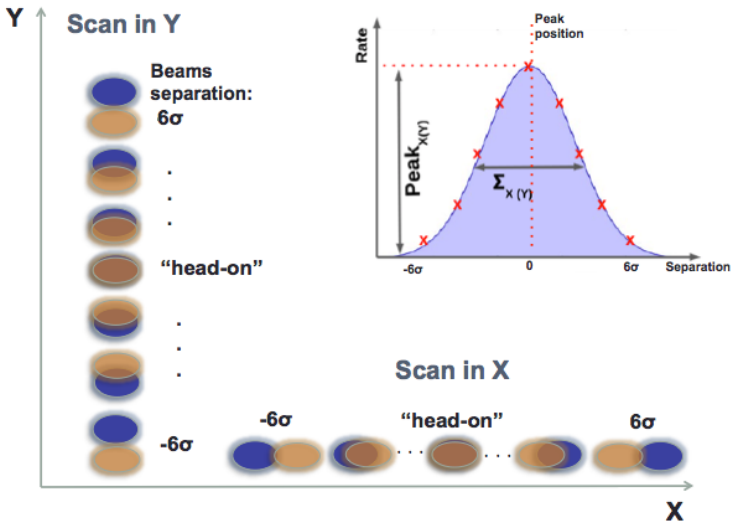
\includegraphics[scale=.37]{Chapter3/vdm_sketch.png}
    \caption[Sketch of a vdM scan in X and Y planes and example of fitting resulting rates]{ The sketch of a vdM scan in X and Y planes. The indent sketch is an example of the fitting of the resulting rates \cite{vdM_sketch}.}
    \label{vdm_sketch}
  \end{figure}
\end{center}




% https://pos.sissa.it/364/194/pdf



\subsection*{Backgrounds}



